\documentclass{beamer}
\usetheme{Madrid} % Choose your favorite theme here

% Packages
\usepackage{graphicx}
\usepackage{amsmath}
\usepackage{caption}
\usepackage{subcaption}

% Title page
\title[NCAA Basketball Analysis]{NCAA Basketball Analysis}
\author[STAT 386]{Maclean Sherren \& Kayla Tansiongco}
\institute[Brigham Young University]{Brigham Young University}
\date{\today}

\begin{document}

\begin{frame}
\titlepage
\end{frame}

\begin{frame}{Outline}
\tableofcontents
\end{frame}

\section{Introduction}

\begin{frame}{Introduction}
\begin{itemize}
  \item Due to Covid, 2020 NCAA tournament did not happen.
  \item Question: Are there certain regular season variables that are better predictors for postseason outcomes?
  \item Goal: Use existing data/trends from other years and regular season data from 2020 to come up with potential methods of prediction and postseason outcomes.
\end{itemize}
\end{frame}

\section{Data Collection}

\begin{frame}{Data Collection}
\begin{itemize}
  \item College Basketball Dataset folder found on Kaggle. Dataset "cbb.csv" has regular and postseason statistics from years 2013-2021. Excludes 2020 season due to lack of postseason statistics.
  \item Folder included datasets for each individual year, with 2020 ("cbb20.csv") having regular season stats only.
  \item Variables of final dataset: YEAR, TEAM, CONF, G, W, BARTHAG, \textcolor{blue}{POSTSEASON}, \textcolor{blue}{SEASON\_FINAL}.
\end{itemize}
\end{frame}

\begin{frame}{Data Collection}
\begin{itemize}
  \item Created numerically coded column, SEASON\_FINAL, derived from POSTSEASON (string data type) for cbb.csv dataframe. (Ex: "Champions" = 1, "2ND" = 2, "F4" = 4)
  \item Initialized variables POSTSEASON and SEASON\_FINAL as NaN for cbb20.csv dataframe. This is what we will fill in through our prediction methods.
\end{itemize}
\end{frame}

\section{Exploratory Data Analysis}

\begin{frame}{Exploratory Data Analysis}
\begin{itemize}
  \item Determine what variables are most correlated with POSTSEASON outcomes.
  \item Used Spearman correlation since it is more appropriate for measurements taken from ordinal scales.
\end{itemize}
\end{frame}

\begin{frame}{Exploratory Data Analysis}
  \begin{center}
    \begin{itemize}
        \item BARTHAG vs SEASON\_FINAL
        \item BARTHAG = Power Rating (Chance of beating an average Division 1 team)
    \end{itemize}

    \begin{figure}
      \centering
      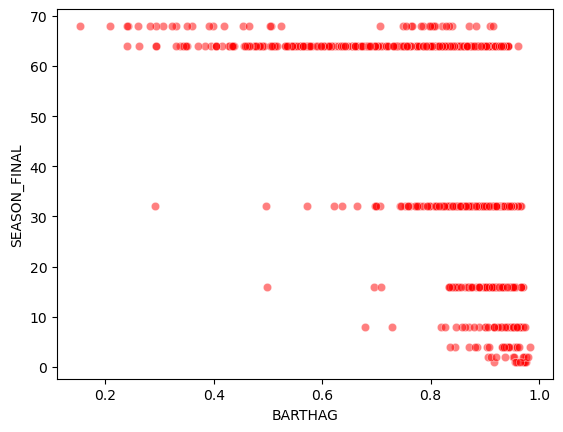
\includegraphics[width=0.5\linewidth]{barthagscatterplot.png} % Replace with barthagscatterplot
    \end{figure}

    \vspace{0.1cm}

    Corr: -0.6461273899341722
  \end{center}
\end{frame}

\begin{frame}{Exploratory Data Analysis}
  \begin{center}
    \begin{itemize}
        \item W vs SEASON\_FINAL
        \item W = Number of games won
    \end{itemize}

    \begin{figure}
      \centering
      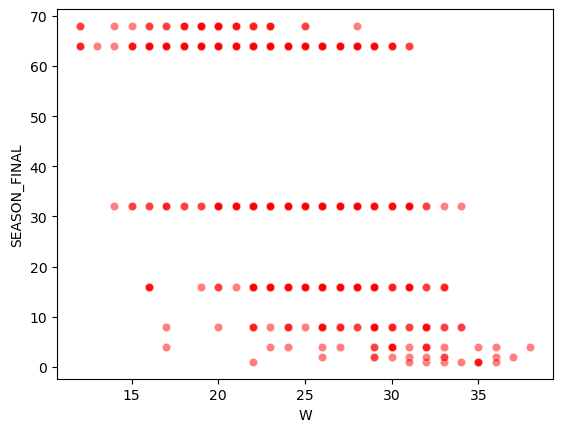
\includegraphics[width=0.5\linewidth]{wscatterplot.png} % Replace with w scatterplot
    \end{figure}

    \vspace{0.1cm}

    Corr: -0.5125436890870254
  \end{center}
\end{frame}

\begin{frame}{Exploratory Data Analysis}
  \begin{center}
    \begin{itemize}
        \item W/L vs SEASON\_FINAL
        \item W/L = Win-Loss Ratio
    \end{itemize}

    \begin{figure}
      \centering
      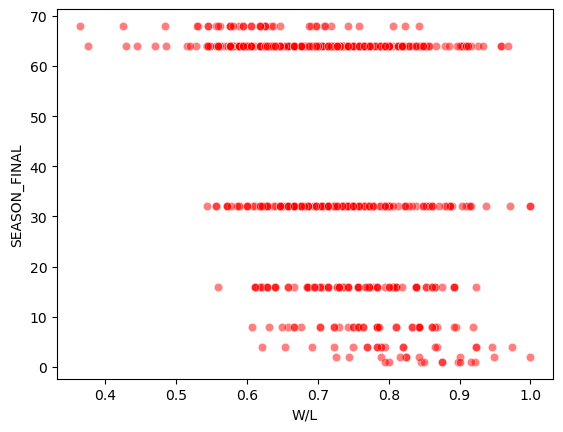
\includegraphics[width=0.5\linewidth]{wlscatterplot.png} % Replace with w/l scatterplot
    \end{figure}

    \vspace{0.1cm}

    Corr: -0.3532346489556209

  \end{center}
\end{frame}

\begin{frame}{Exploratory Data Analysis}
  \begin{center}
    \begin{itemize}
        \item SEED vs SEASON\_FINAL
        \item SEED = Seed in the NCAA March Madness Tournament
    \end{itemize}

    \begin{figure}
      \centering
      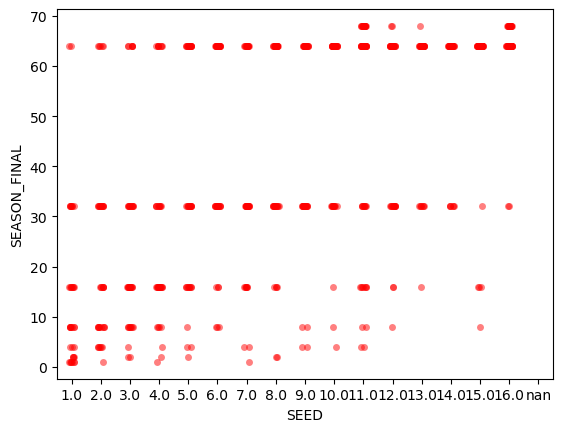
\includegraphics[width=0.5\linewidth]{seedscatterplot.png} % Replace with seed scatterplot
    \end{figure}

    \vspace{0.1cm}

    Corr: 0.6065146756151623
  \end{center}
\end{frame}

\section{Methodology}

\begin{frame}{Methodology}
\begin{itemize}
  \item Package contains a function that takes a season and method of prediction, then produces simulated results of an NCAA tournament.
  \item Compare predicted results to actual results.
  \item Create a prediction for 2020 NCAA postseason tournament.
  \item Since seeding was not determined for 2020 postseason, variable RK will be used as a predictor.
\end{itemize}
\end{frame}

\begin{frame}{Methodology}
\begin{itemize}
  \item Season: 2021
  \item Method: BARTHAG (Power Rating)
\end{itemize}

\begin{columns}[T] % Align columns at the top
\begin{column}{0.5\textwidth} % Left column
  \textbf{Predicted Final Four}
  \begin{itemize}
    \item Baylor
    \item Michigan
    \item Gonzaga
    \item Houston
  \end{itemize}
  \textbf{Predicted Championship}
  \begin{itemize}
    \item Gonzaga vs Baylor
    \item Winner: Baylor
    \end{itemize}
\end{column}
\begin{column}{0.5\textwidth} % Right column
  \textbf{Actual Final Four}
  \begin{itemize}
    \item Baylor
    \item Gonzaga
    \item Houston
    \item UCLA
  \end{itemize}
  \textbf{Actual Championship}
  \begin{itemize}
  \item Gonzaga vs Baylor
  \item Winner: Baylor
  \end{itemize}
\end{column}
\end{columns}
\end{frame}

\begin{frame}{Methodology}
\begin{itemize}
  \item Season: 2021
  \item Method: W (Wins)
\end{itemize}

\begin{columns}[T] % Align columns at the top
\begin{column}{0.5\textwidth} % Left column
  \textbf{Predicted Final Four}
  \begin{itemize}
    \item Winthrop
    \item Alabama
    \item Gonzaga
    \item Loyola Chicago
  \end{itemize}
  \textbf{Predicted Championship}
  \begin{itemize}
    \item Alabama vs Gonzaga
    \item Winner: Alabama
    \end{itemize}
\end{column}
\begin{column}{0.5\textwidth} % Right column
  \textbf{Actual Final Four}
  \begin{itemize}
    \item Baylor
    \item Gonzaga
    \item Houston
    \item UCLA
  \end{itemize}
  \textbf{Actual Championship}
  \begin{itemize}
    \item Gonzaga vs Baylor
    \item Winner: Baylor
    \end{itemize}
\end{column}
\end{columns}
\end{frame}

\begin{frame}{Methodology}
\begin{itemize}
  \item Season: 2021
  \item Method: SEED
\end{itemize}

\begin{columns}[T] % Align columns at the top
\begin{column}{0.5\textwidth} % Left column
  \textbf{Predicted Final Four}
  \begin{itemize}
    \item Baylor
    \item Gonzaga
    \item Michigan
    \item Illinois
  \end{itemize}
  \textbf{Predicted Championship}
  \begin{itemize}
    \item Michigan vs Gonzaga
    \item Winner: Gonzaga
    \end{itemize}
\end{column}
\begin{column}{0.5\textwidth} % Right column
  \textbf{Actual Final Four}
  \begin{itemize}
    \item Baylor
    \item Gonzaga
    \item Houston
    \item UCLA
  \end{itemize}
  \textbf{Actual Championship}
  \begin{itemize}
    \item Gonzaga vs Baylor
    \item Winner: Baylor
    \end{itemize}
\end{column}
\end{columns}
\end{frame}

\section{Results}

\begin{frame}{Results}
\begin{itemize}
  \item Season: 2020 
  \item Method: BARTHAG (Power Rating)
  
      \begin{figure}
      %\centering
      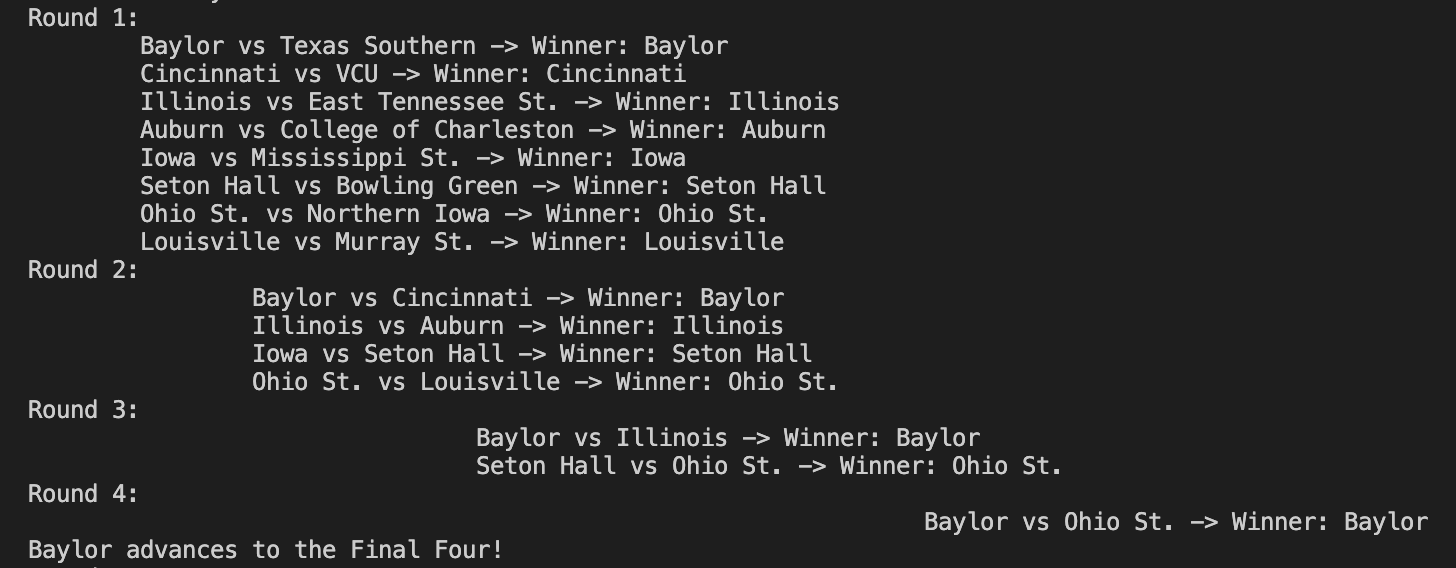
\includegraphics[width=0.7\linewidth]{CBB2020_power_south16.png}
      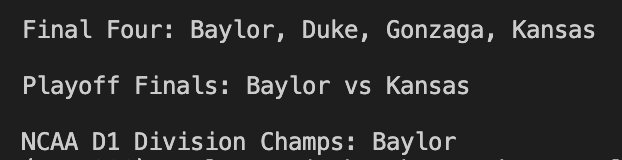
\includegraphics[width=0.7\linewidth]{CBB2020_power_final.png}
    \end{figure}
    
\end{itemize}
\end{frame}

\begin{frame}{Results}
\begin{itemize}
  \item Season: 2020 
  \item Method: W (Wins)
  
      \begin{figure}
      %\centering
      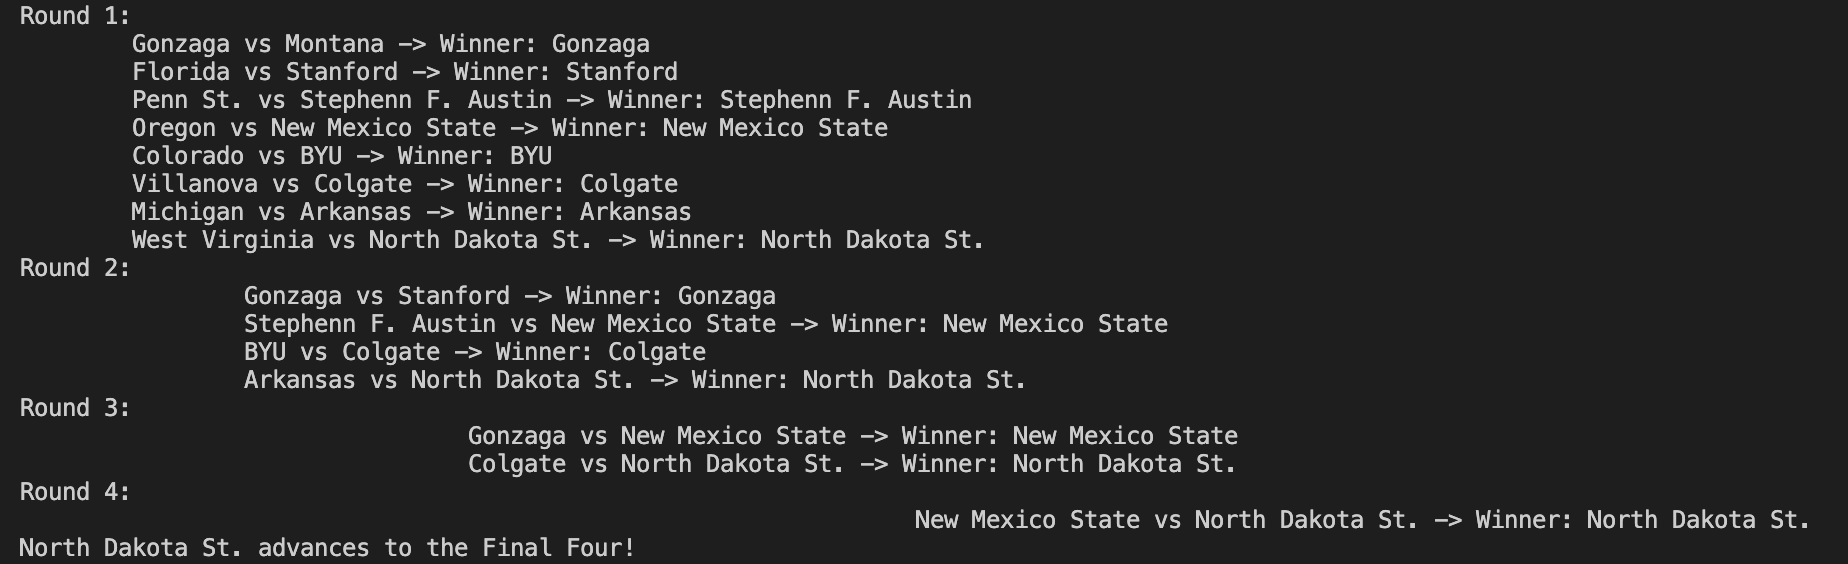
\includegraphics[width=0.4\linewidth]{CBB2020_wins_west16.png}
      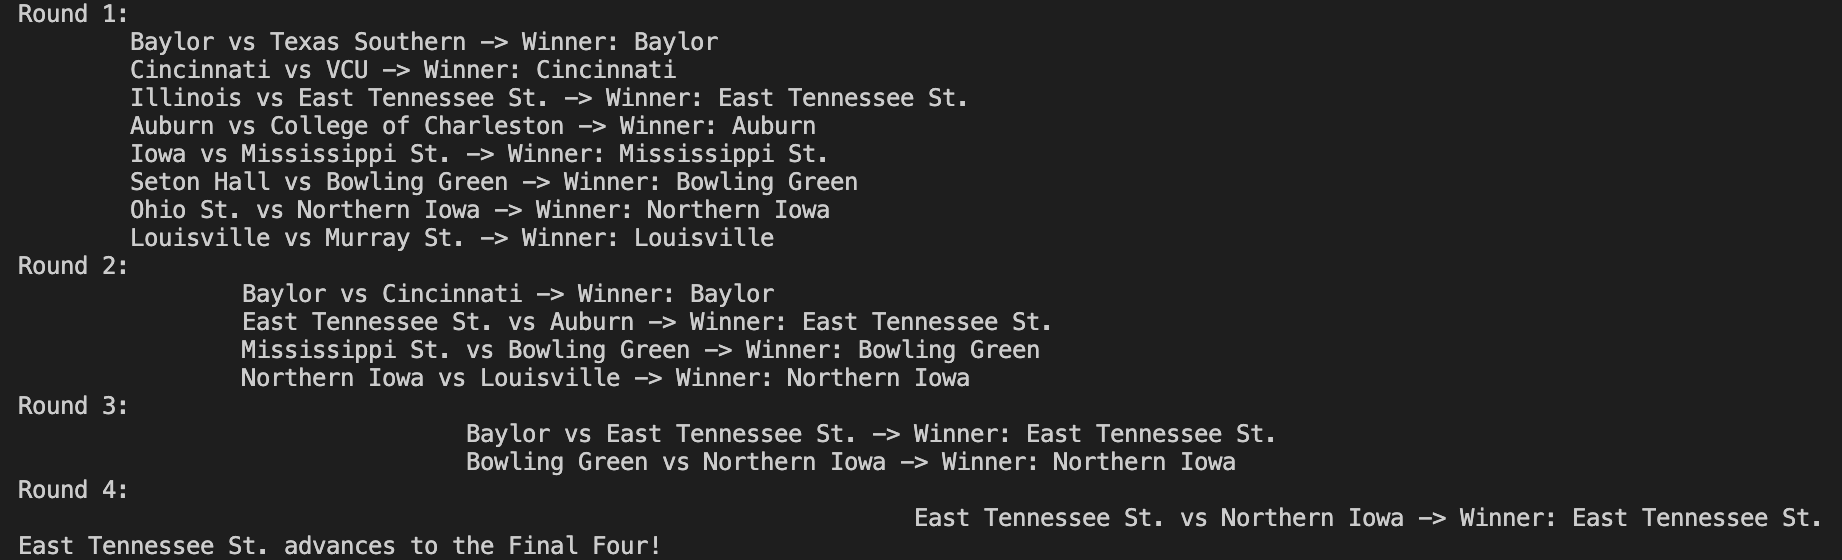
\includegraphics[width=0.4\linewidth]{CBB2020_wins_south16.png}
      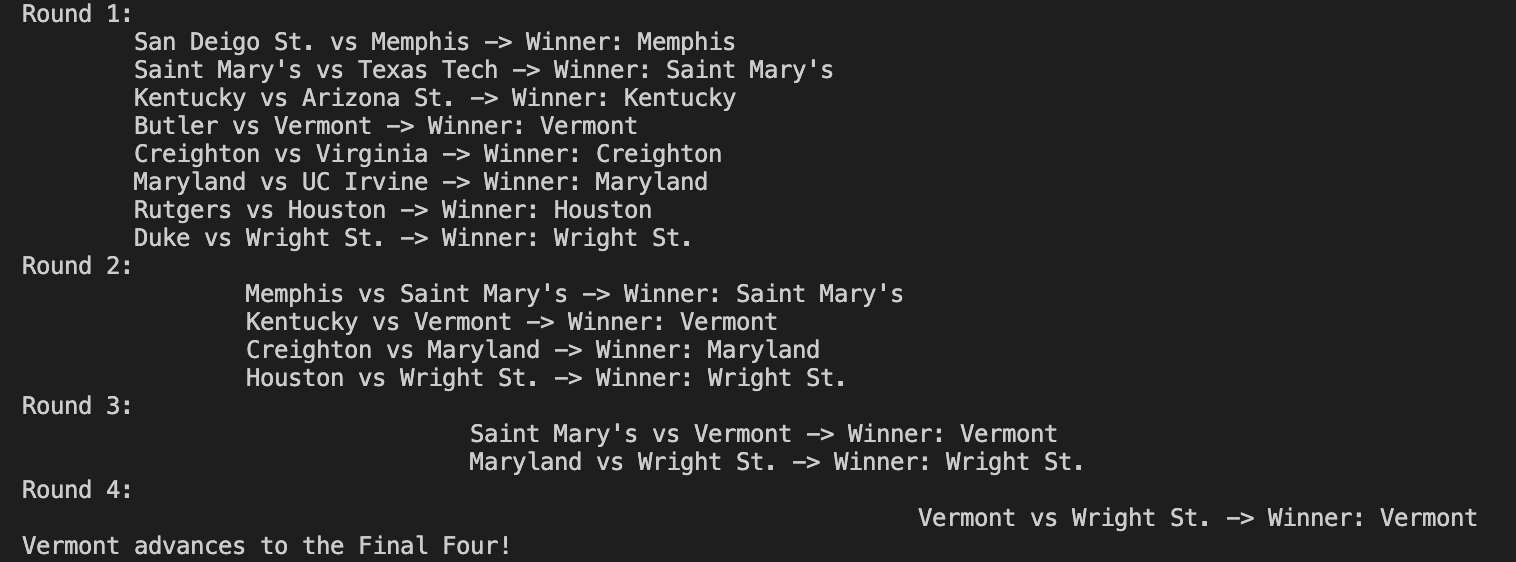
\includegraphics[width=0.4\linewidth]{CBB2020_wins_east16.png}
      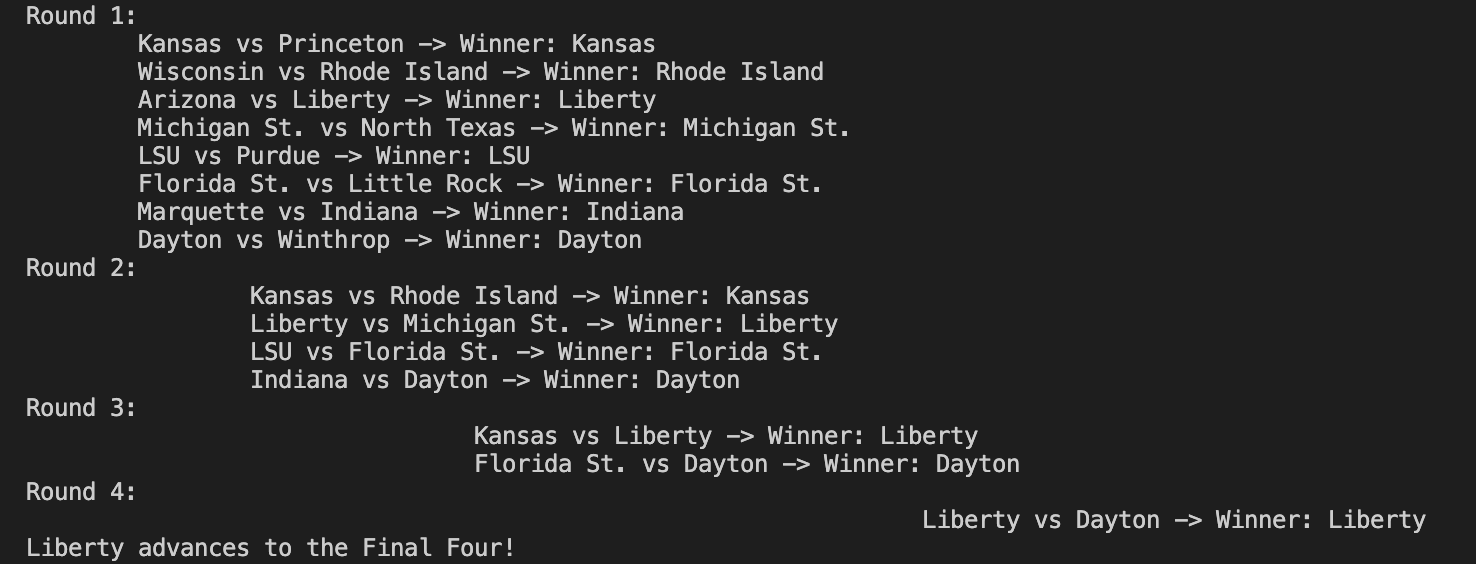
\includegraphics[width=0.4\linewidth]{CBB2020_wins_midwest16.png}
      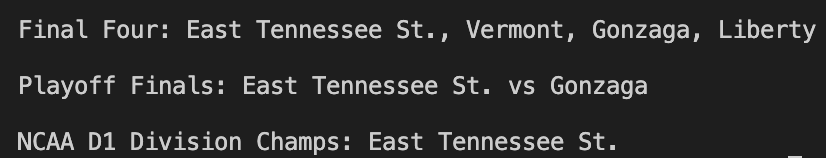
\includegraphics[width=0.6\linewidth]{CBB2020_wins_final.png}    
    \end{figure}
\end{itemize}
\end{frame}

\begin{frame}{Results}
\begin{itemize}
  \item Season: 2020 
  \item Method: RK (Rank/Equivalent to SEED)
  
      \begin{figure}
      %\centering
      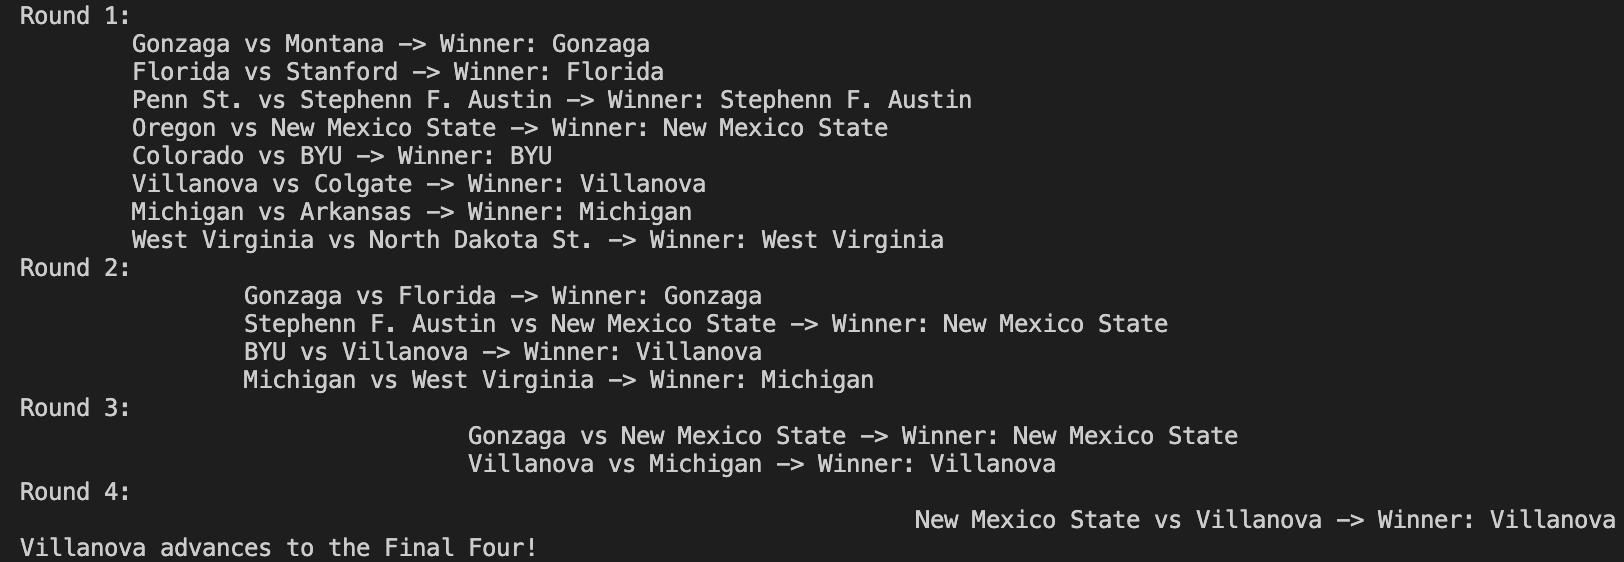
\includegraphics[width=0.4\linewidth]{CBB2020_rank_west16.png}
      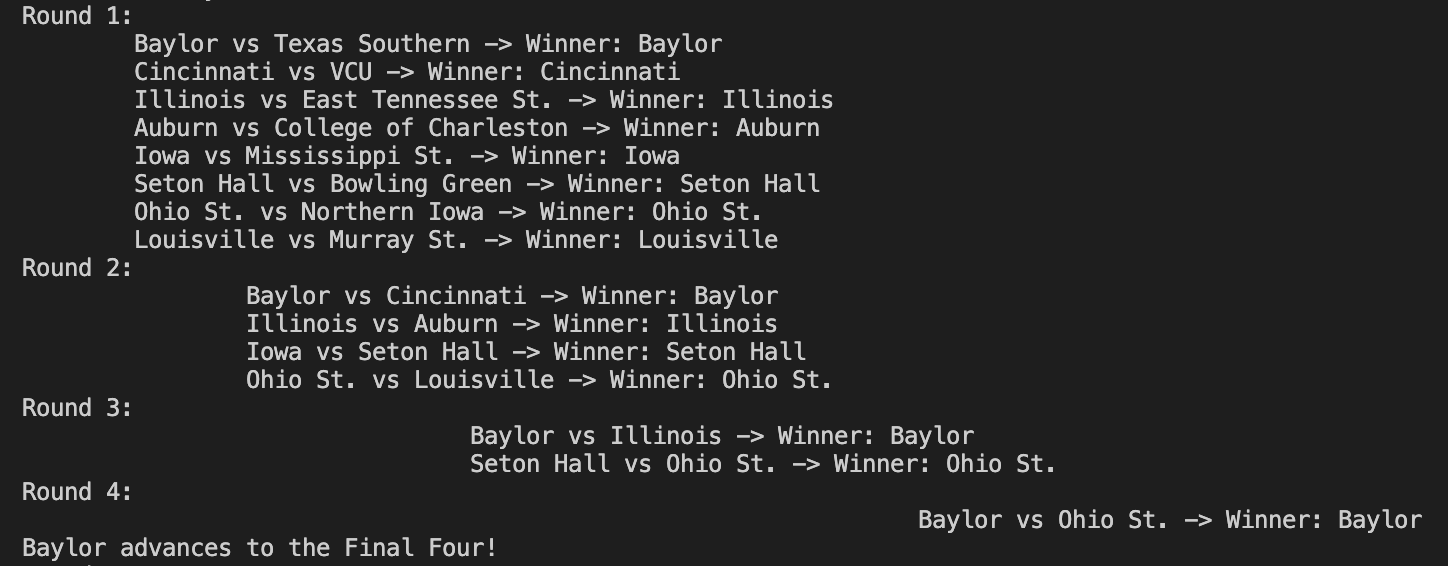
\includegraphics[width=0.4\linewidth]{CBB2020_rank_south16.png}
      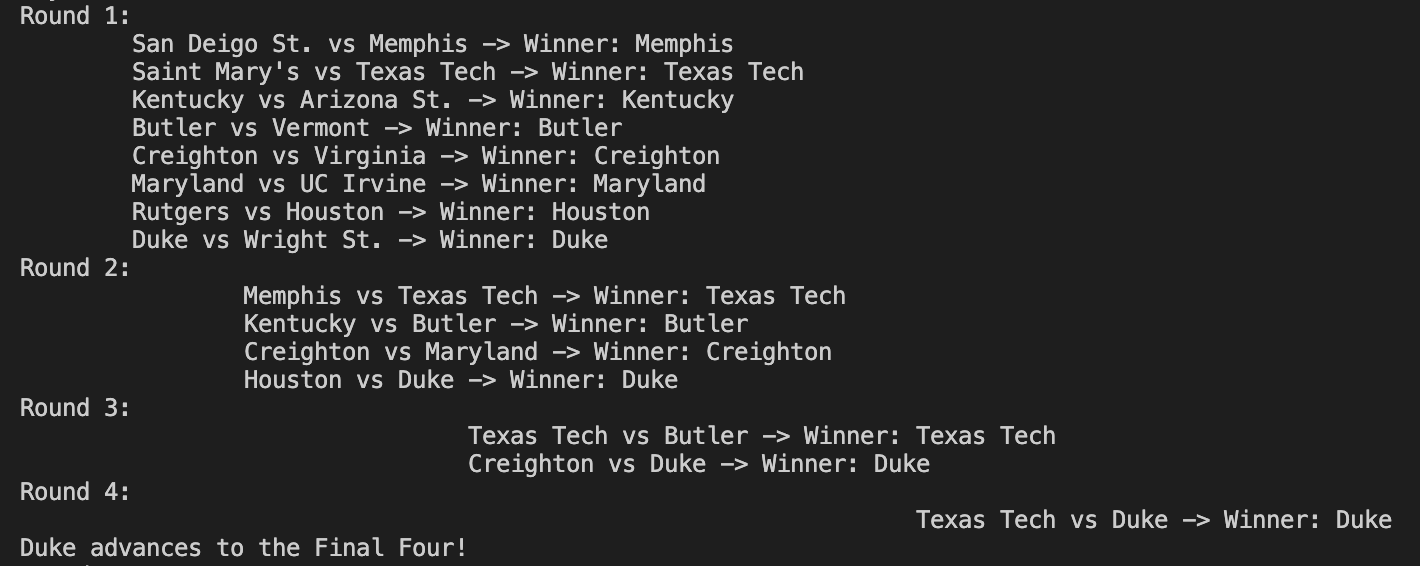
\includegraphics[width=0.4\linewidth]{CBB2020_rank_east16.png}
      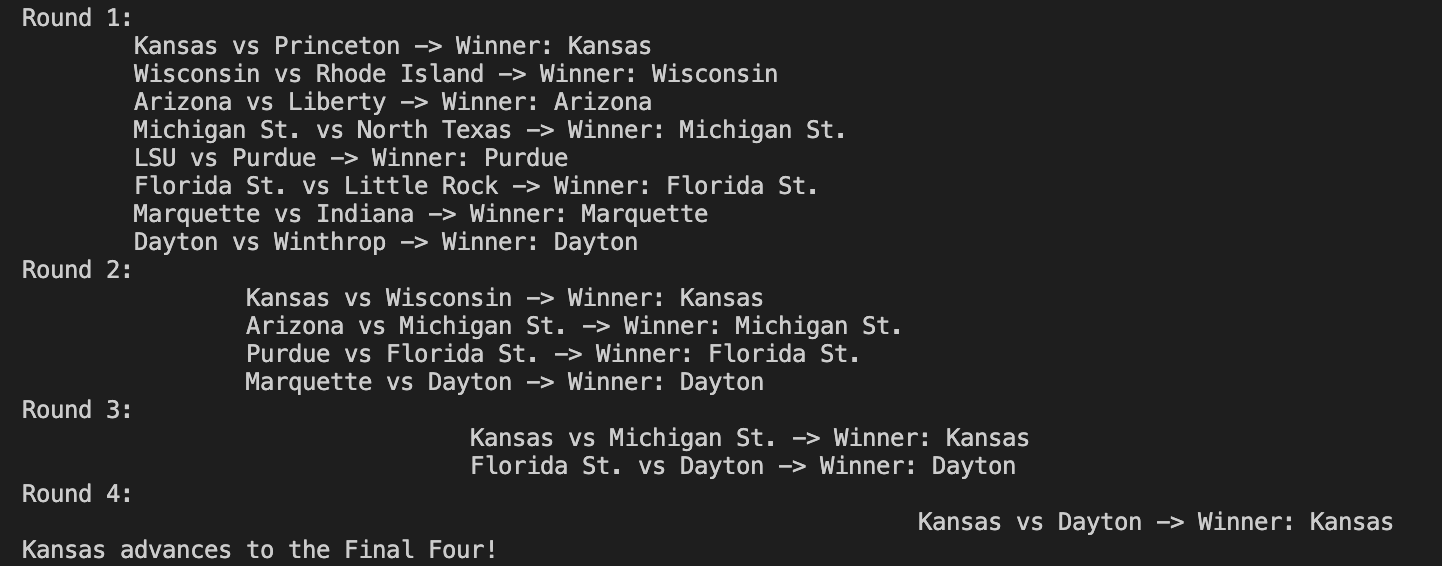
\includegraphics[width=0.4\linewidth]{CBB2020_rank_midwest16.png}
      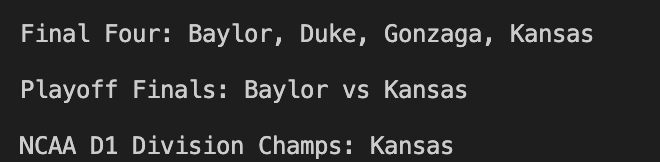
\includegraphics[width=0.6\linewidth]{CBB2020_rank_final.png}    
      \end{figure}
    
\end{itemize}
\end{frame}

\section{Conclusion}

\begin{frame}{Conclusion}
\begin{itemize}
  \item While there is a lot of randomness and uncertainty to account for in the NCAA tournament, there are variables that can accurately predict the outcomes.
  \item Among the variables observed, power rating was the strongest method of prediction.
  \item Potential to apply package to other variables as well.
  \item Aside from our own observations, we could apply further analyses to evaluate the accuracy of our predictors.
  \item Potential to use same methods to make predictions for future seasons.
\end{itemize}
\end{frame}

\section{Q \& A}

\begin{frame}{Questions \& Answers}
\begin{center}
\Huge Questions or comments?
\end{center}
\end{frame}

\begin{frame}{Thank You}
\begin{center}
\Huge Thank you! Happy Holidays!
\end{center}
\end{frame}

\section{References}
\begin{frame}{References}
  \begin{itemize}
    \item Kaggle Dataset
    \href{https://www.kaggle.com/datasets/andrewsundberg/college-basketball-dataset?select=cbb.csv}{https://www.kaggle.com/datasets/andrewsundberg/college-basketball-dataset?select=cbb.csv}
    \item 2021 NCAA Tournament Results
    \href{https://www.ncaa.com/news/basketball-men/article/2022-07-20/2021-ncaa-bracket-scores-stats-records-march-madness-mens-tournament}{https://www.ncaa.com/news/basketball-men/article/2022-07-20/2021-ncaa-bracket-scores-stats-records-march-madness-mens-tournament}
    \item 2020 Predicted Bracket
    \href{https://www.ncaa.com/news/basketball-men/article/2020-02-28/ncaa-predictions-projections-2020-bracket-andy-katz}{https://www.ncaa.com/news/basketball-men/article/2020-02-28/ncaa-predictions-projections-2020-bracket-andy-katz}
    \item BracketMaker (preliminary guide for package structure)
    \href{https://github.com/klauscurde/BracketMaker}{https://github.com/klauscurde/BracketMaker}
  \end{itemize}
  \end{frame}

\end{document}
